\subsection{BỘ DỮ LIỆU}
Bộ dữ liệu cung cấp thông tin chi tiết dữ liệu giá của 3 kim loại quý, cụ thể là Vàng, Bạch Kim và Palladi trong giai đoạn từ 01/03/2019 đến 26/03/2024. Dữ liệu bao gồm các cột: Ngày (Date), Giá mở cửa (Open), Giá đóng cửa (Close), Giá cao nhất (High), Giá thấp nhất (Low). Do mục tiêu là dự báo giá đóng cửa nên chỉ xử lý dữ liệu liên quan đến cột “Close”.

\subsection{MÔ TẢ THỐNG KÊ}
\begin{table}[htbp]
  \centering
\begin{tabular}{|c|c|c|c|}
    \hline
     \  & Gold & Palladium & Platinum \\ \hline
     Count & 1694 & 1687& 1695\\ \hline
     Mean & 1780,64 & 1888,11 & 958,24\\ \hline
     Std & 197,721 & 507,233 & 105,894\\ \hline
     Min & 1270,65 & 859,5 & 595\\ \hline
     25\% & 1708,035 & 1467 & 892\\ \hline
     50\% & 1811,18 & 1927,5 & 943,5\\ \hline
     75\% & 1923,6 & 2294,25 & 1018,5\\ \hline
     Max & 2202,2 & 3178 & 1306\\ \hline
\end{tabular}
\caption{Mô tả thống kê của vàng, paladi và bạch kim}
\end{table}

\begin{figure}[htbp]
\centerline{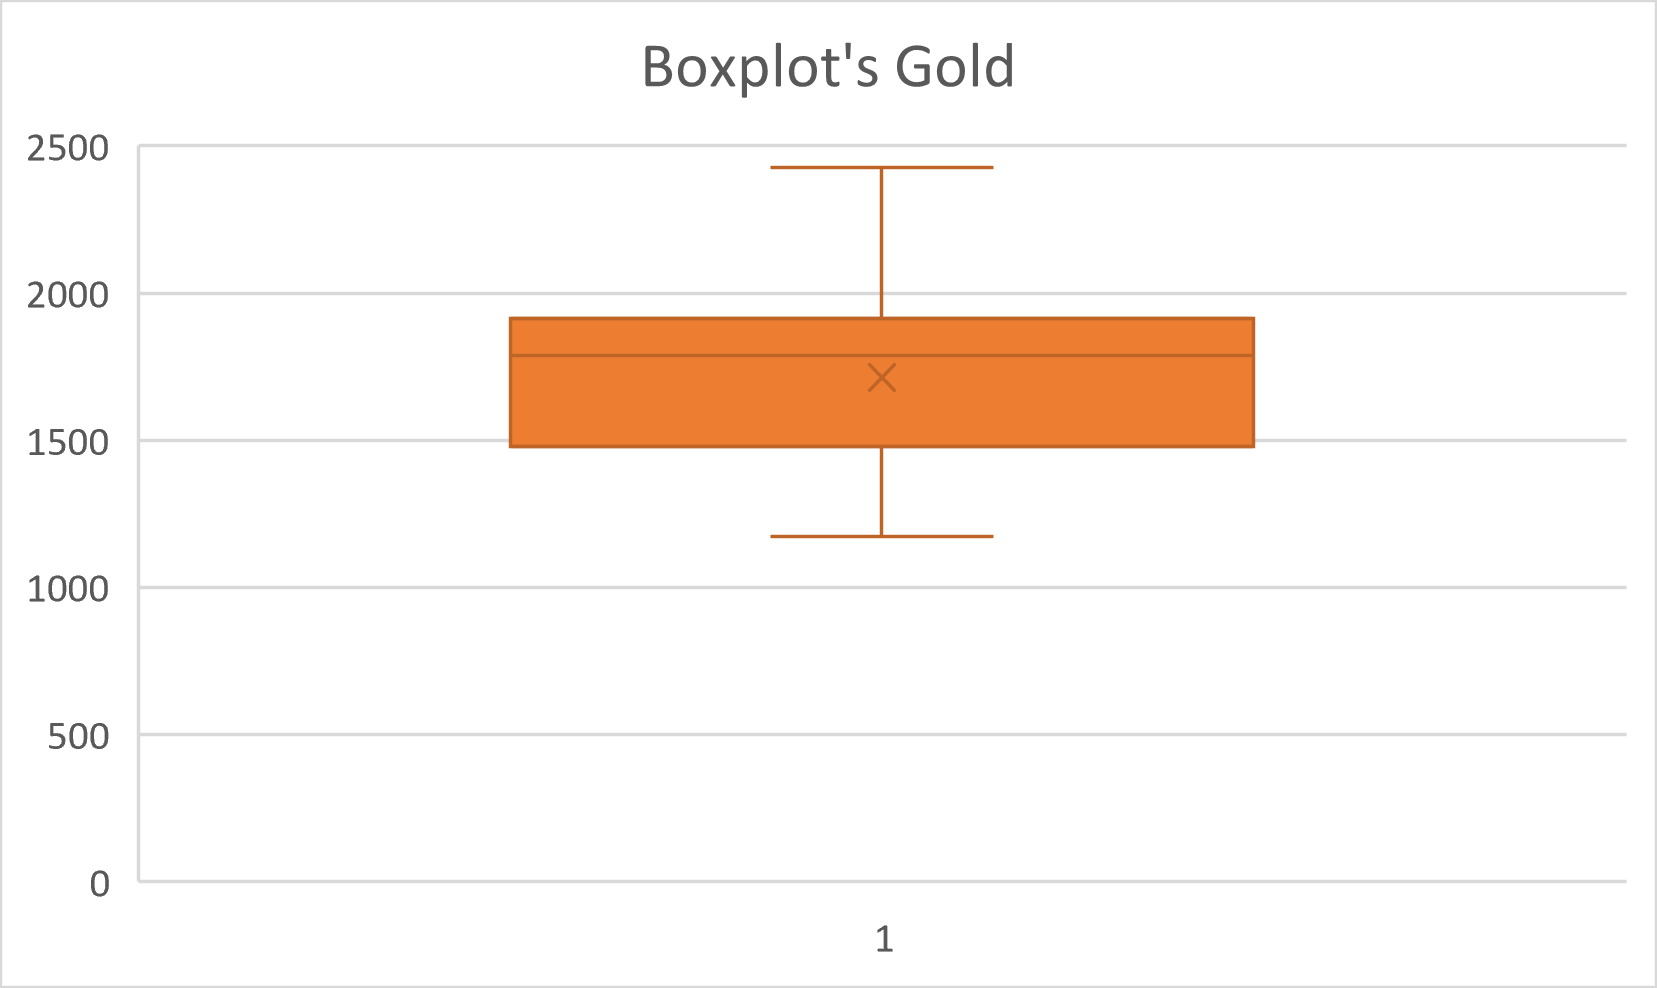
\includegraphics[width=0.4\textwidth]{img/Picture2.png}}
\caption{Sơ đồ boxplot của vàng}
\label{fig}
\end{figure}

\begin{figure}[htbp]
\centerline{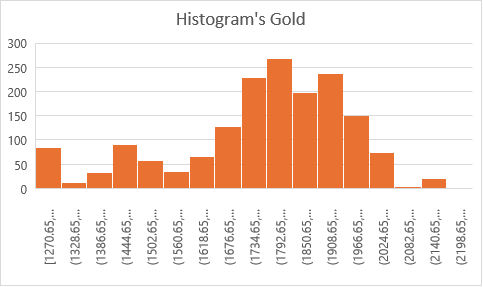
\includegraphics[width=0.4\textwidth]{img/Picture5.png}}
\caption{Sơ đồ histogram của vàng}
\label{fig}
\end{figure}

\begin{figure}[htbp]
\centerline{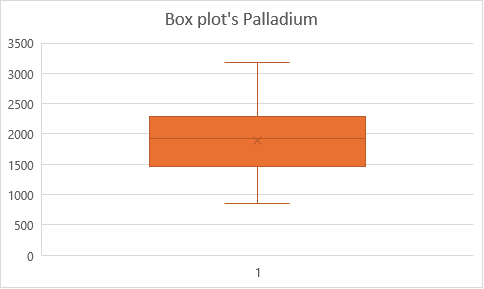
\includegraphics[width=0.4\textwidth]{img/Picture3.png}}
\caption{Sơ đồ boxplot của Paladi}
\label{fig}
\end{figure}

\begin{figure}[htbp]
\centerline{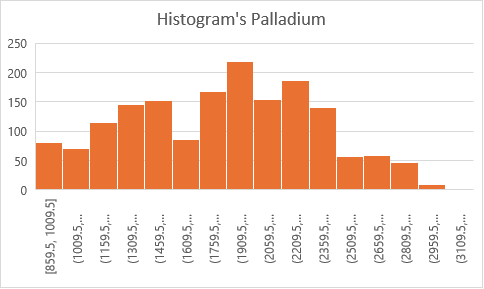
\includegraphics[width=0.4\textwidth]{img/Picture6.png}}
\caption{Sơ đồ histogram của Paladi}
\label{fig}
\end{figure}

\begin{figure}[htbp]
\centerline{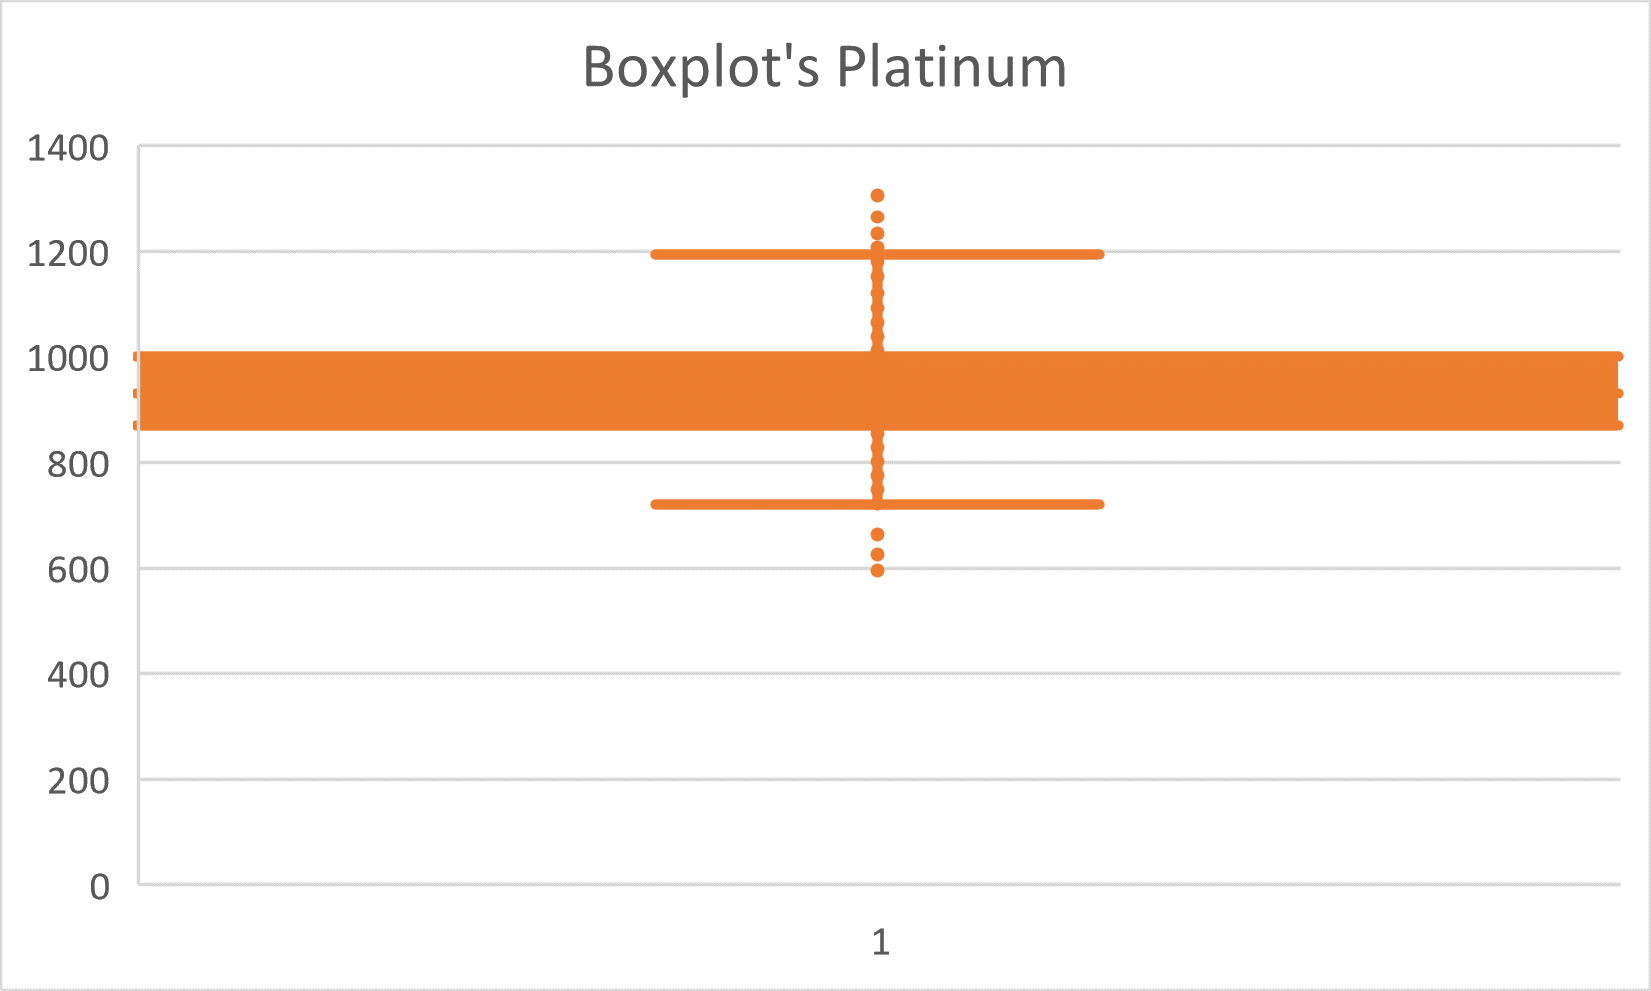
\includegraphics[width=0.4\textwidth]{img/Picture4.png}}
\caption{Sơ đồ boxplot của bạch kim}
\label{fig}
\end{figure}

\begin{figure}[htbp]
\centerline{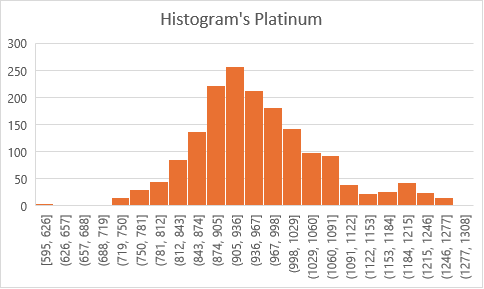
\includegraphics[width=0.4\textwidth]{img/Picture7.png}}
\caption{Sơ đồ histogram của bạch kim}
\label{fit}
\end{figure}